\chapter{Obserwacje i wyniki}
Przeprocesowanie dostarczonego zbioru danych zajęło 11 dni, co poskutkowało zebraniem około 30GB informacji na temat analizowanych domen.

\section{Typy odebranych odpowiedzi}
Wśród przeanalizowanych par domen i serwerów można zaobserwować kilka charakterystycznych typów odpowiedzi. Odpowiedzi mogą być dzielone na kategorie ze względu na różne kryteria. Pierwszym kryterium, które będzie brane pod uwagę w niniejszej pracy jest po prostu rozmiar pliku przechowującego informacje pobrane z serwera autorytatywnego. Jest to motywowane faktem, że w istocie im większy jest plik z odpowiedzią, tym spodziewamy się, że zawiera on więcej informacji na temat odpytywanej domeny. 

Pierwszym typem jest odpowiedź, która zajmowała na dysku specyficzną ilość miejsca -- 25123 bajty. Zaobserwowano, że uzyskano 626288 odpowiedzi tego typu. Rozmiar pliku jest swego rodzaju skutkiem ubocznym uproszczonej implementacji skanera. Trudno było przewidzieć wszystkie specyficzne przypadki towarzyszące transferowi strefy DNS. Zaobserwowana sytuacja jest właśnie jednym z tych nietypowych sytuacji i nawet program dig nie odzworowuje idealnie zachowania jakie powinno nastąpić w takiej sytuacji. przyczyna utworzenia opisanego wcześniej pliku nie jest jednoznacznie określona. Zostały podjęte próby ustalenia czym spowodowane jest takie zachowanie. W takich samych przypadkach program dig zwraca jedynie rekord DNS SOA i komunikat o błędzie (ang. \textit{communications error: end of file}). Zachowanie programu dig w dużym stopniu przypomina przekierowanie zapytania IXFR na AXFR (ang. \textit{AXFR fallback}) opisane między innymi w RFC1995\cite{RFC1995}. Wywołanie mechanizmu AXFR fallback następuje w sytuacji, kiedy numer wersji pliku strefy przysłany do serwera jest wyższy niż numer wersji aktualnie na nim przechowywany. Na różnego rodzaju forach\cite{powerdns-forum} czy w serwisach internetowych\cite{powerdns-git}, problem który został opisany pojawia się najczęściej jako problem implementacji oprogramowania PowerDNS\cite{powerdns}. Niemniej jednak nie ustalono dokładnie jaki jest powód wysłania tak dużego pakietu w odpowiedzi na zwykłe zapytanie AXFR.

Kolejnym przykładem odpowiedzi, która powodowała powstanie dużego pliku na dysku, było odebranie od serwera autorytatywnego pakietu TCP RST(ang. \textit{TCP reset packet}). Sytuacja taka wynika również z pewnego uproszczenia, które zostało przyjęte w implementacji skanera. Założono, że zawsze zostanie odebrany pakiet DNS. Podyktowane było to ograniczonym czasem w którym implementowano skaner oraz faktem, że problem ten można w łatwy sposób obejść poprzez odfiltrowanie odpowiednich plików w katalogu z wynikami. Dodatkowo sytuacje tego typu były bardzo sporadyczne, więc nie afektowało to w znaczącym stopniu ani na czas przeanalizowania pobranych danych ani na wynik tej analizy.

Kolejnymi specyficznymi grupami jeśli chodzi o rozmiar pliku z odpowiedzią są już typowe odpowiedzi na zapytania AXFR. Najmniejzy rozmiar mają oczywiście odpowiedzi, które zawierają jedynie rekord SOA i jest to dopuszczalna odpowiedź na zapytanie AXFR. Następnie, wraz ze zwiększającą się liczbą wpisów w pliku strefy DNS, zwiększa się rozmiar odpowiedzi. Nie przekłada się to jednak bezpośrednio na informacje, które można wyodrębnić z takich plików strefy. Zdarza się bowiem sytuacja, w której znaczną część pliku strefy DNS zajmują wpisy podpisów cyfrowych RRSIG, których długość przekłada się na rozmiar plików. Dodatkowo, podpisy generowane mogą być dla każdego rekordu oddzielnie (co szerzej opisano w podpunkcie \ref{RSIG}), dlatego też wpływa to bardzo znacząco na rozmiar otrzymywanej odpowiedzi.

\section{Odebrane adresy IPv4}
Częstym argumentem, który pojawia się podczas dyskusji na temat bezpieczeństwa transferów plików bazy danych DNS jest ujawnianie adresów IP. W niniejszym podrozdziale skupiono się głównie na adresach IP w wersji 4. ponieważ jest to wciąż dominujący typ adresacji w Internecie. Okazuje się, że pomimo obaw o wycieki adresów przez dokonywanie nieuprawnionego transferu nikt nie zbadał dokładnie jak duża może być skala tego zjawiska. Umożliwiły to badania przeprowadzone w tej pracy magisterskiej.

Po przeprowadzeniu skanowania okazało się, że dzięki przeprowadzonemu skanowaniu uzyskano informację o ponad <123456789> publicznych adresach IP w wersji 4. 

\section{Analiza TLD}
Jednym z podejść analizy zebranego zbioru danych było sprawdzenie, jak przedstawia się rozkład popularności domeny najwyższego poziomu dla serwerów podatnych na nieuprawiony transfer strefy. 

W głównej mierze należy zastanowić się, czy rozkład ten jest w ogóle istotny, czy może nie różni się on niczym od ogólnego, całościowego rozkładu popularności TLD w internecie, bez uwzględnienia podatności czy innych czynników. W tym celu przeanalizowano i przedstawiono wykres popularności domen najwyższego poziomu w sieci internet. Jest on przedstawiony na rysunku \ref{TLD_all}.
\begin{center}
	\begin{figure}
		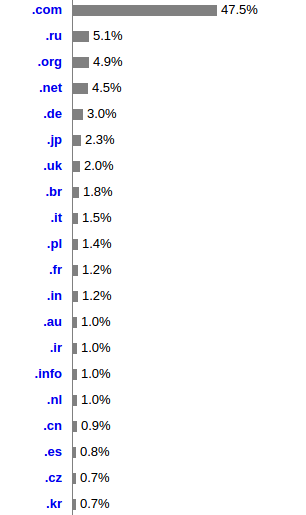
\includegraphics[scale=0.75]{image/TLD_all}\label{TLD_all}
		\caption{Popularność TLD w internecie (dostęp na dzień 15. maja 2017), źródło:  \cite{TLD_popularity}}
	\end{figure}
\end{center}  

Wykres przedstawia procentowy rozkład poszczególnych domen internetowych w zależności od używanej domeny najwyższego poziomu. Wynika z niego, że domena najwyższego poziomu \textit{.com} jest używana przez 47.5\% wszystkich domen. Wykres ograniczony został do 20 najbardziej popularnych TLD. Różnice pomiędzy kolejnymi rekordami są na tyle niskie, że ich umieszczenie wpływałoby negatywnie na ogólną rezprezentację wyników. Wykres \ref{TLD_all} zostanie następnie zestawiony z popularnością TLD tych domen, których serwery autorytatywne umożliwiają nieuprawniony transfer AXFR. Rozkład popularności TLD domen odpowiadających na zapytanie AXFR przedstawiono na rysunku \ref{resp}.
\begin{center}
	\begin{figure}
		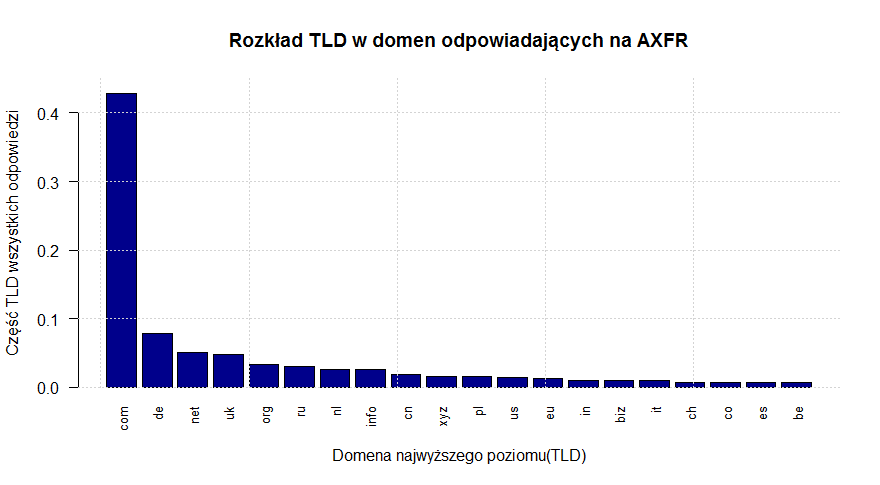
\includegraphics[width=1.0\textwidth]{image/resp}\label{resp}
		\caption{Popularność TLD w odpowiedziach AXFR.}
	\end{figure}
\end{center} 

Dokonując porównania wykresów \ref{TLD_all} oraz \ref{resp} możemy dostrzec kilka prawidłowości. Zarówno w jednym jak i drugim przypadku, wyraźnie dominującą domeną najwyższego poziomu jest domena .com. Dodatkowo, nie można mówić tu o anomalii, ponieważ zarówno w jednym jak i drugim przypadku domena .com stanowi bardzo podobny procentowy udział wszystkich domen, czy to pytanych czy tych, które odpowiedziały. Następnie można dostrzec delikatne zmiany w procentowych udziałach kolejnych TLD, jednak nie na pierwszy rzut oka zmiany te nie są wyróżniające się czy nad wyraz zauważalne.

W związku z tym, że wyżej opisane działania nie pozwoliły na wyraźne zarysowanie różnic pomiędzy rozkładami TLD, zdecydowano się zestawić ze sobą inne zbiory danych. Wykreślono podobne wykresy dla popularności domeny najwyższego poziomu dla domen odpytywanych podczas skanowania oraz TLD domen, które na zapytania odpowiedziały. Następnie zestawiono ze sobą wyniki pozyskane z obu tych zbiorów danych. Zostały odpowiednio wykreślone:
\begin{enumerate}
	\item wykres 15 najpopularniejszych TLD w zbiorze domen odpytywanych w porównaniu do popularności tych TLD w zbiorze domen które odpowiedziały na zapytanie AXFR -- wykres \ref{req_to_resp},
	\item wykres 15 najpopularniejszych TLD w zbiorze domen które odpowiedziały na zapytanie AXFR w zestawieniu z ich popularnością w puli TLD domen odpytywanych -- wykres \ref{resp_to_req}.
\end{enumerate}

\begin{figure}[ht]
	\centering
	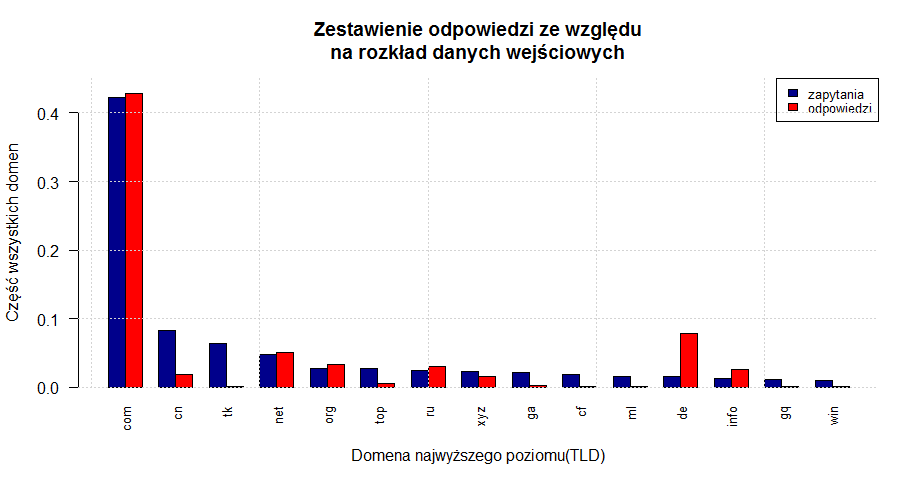
\includegraphics[width=1.0\textwidth]{image/req_to_resp}
	\caption{}
	\label{req_to_resp}
\end{figure}

\begin{figure}[ht]
	\centering
	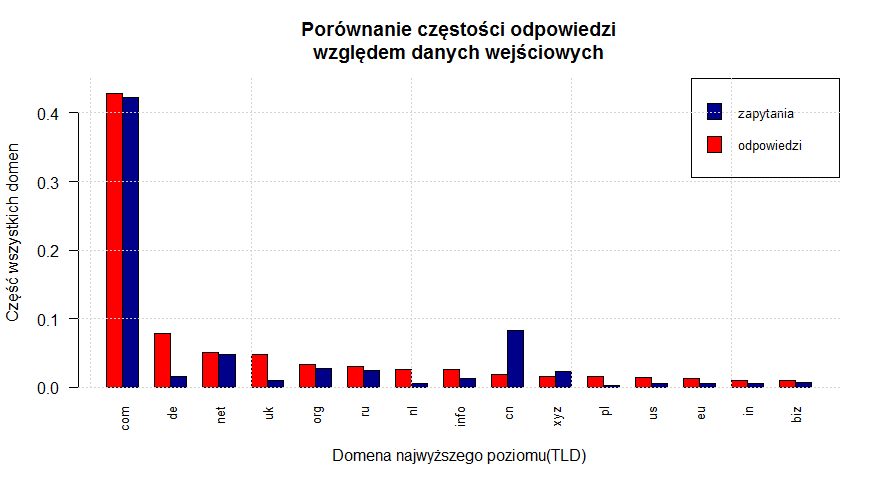
\includegraphics[width=1.0\textwidth]{image/resp_to_req}
	\caption{}
	\label{resp_to_req}
\end{figure}

W przypadku tych bezpośrednich zestawień, można zauważyć więcej interesujących prawidłowości. Na początku warto wspomnieć, że istnieje duża dysproporcja w przypadku niektórych domen najwyższego poziomu. Pierwszą z nich może być przypadek domeny .de, gdzie procentowy udział TLD .de we wszystkich TLD odpowiedzi AXFR jest drugim wynikiem podczas gdy w populacji danych wejściowych jest to 12 najliczniejsza grupa. Warto dodać, że domena .de jest jedną z domen, których zarządcy traktują proceder \textit{zone enumeration} jako łamanie prawa, co opisano w podpunkcie \ref{zone_enumeration}. Transfer AXFR pozwala na uzyskanie danych o podobnej charakterystyce, a mimo to, ok 8\% wszystkich odpowiedzi powiązane jest z domeną najwyższego poziomu .de (domena regionalna -- Niemcy). Podobna sytuacja ma miejsce również w przypadku TLD .uk (Wielka Brytania) czy .pl (Polska), gdzie przy małym współczynniku domen odpytywanych otrzymano nieproporcjonalnie wysoki współczynnik odpowiedzi.

Zjawiskiem w pewnym stopniu odwrotnym do opisanego w poprzednim akapicie jest rozład zapytań/odpowiedzi dla TLD .cn (Chiny) lub .tk (Tokelau -- region zależny od Nowej Zelandii). W tym przypadku zauważalna jest również duża dysproporcja, jednak ,,na korzyść'', gdyż w stosunku do wielu zapytań wystosowanych do domen należących do tych TLD uzyskano relatywnie mało odpowiedzi. Dodatkowo, do grupy opisywanej w tym akapicie można zaliczyć również TLD .top, która została oficjalnie wydzielona w 2014 roku. (... ?)

Oprócz opisanych wcześniej względnych porównań pomiędzy pytaniami i odpowiedziami od serwerów autorytatywnych różnych domen sprawdzono jak wygląda dystrybuanta poszczególnych rozkładów. Pozowliło to oszacować ile (ilościowo) domen najwyższego poziomu zawierało się w grupie, dla której generowano większość zapytań (rysunek \ref{cdf_tld_req}). Analogicznie, w przypadku danych dotyczących odpowiedzi AXFR można było ocenić ile różnych TLD pojawia się niemal we wszystkich odpowiedziach (rysunek \ref{cdf_tld_resp}).

\begin{figure}[ht]
	\centering
	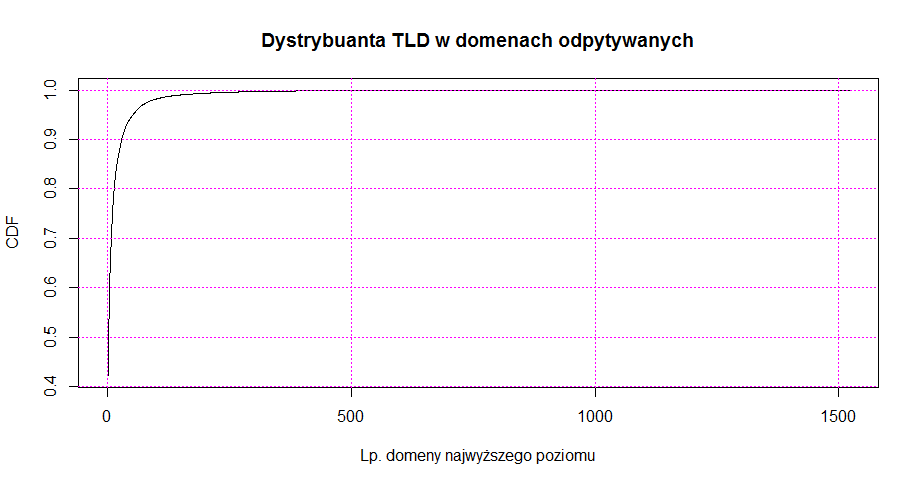
\includegraphics[width=1.0\textwidth]{image/cdf_tld_req}
	\caption{}
	\label{cdf_tld_req}
\end{figure}

\begin{figure}[ht]
	\centering
	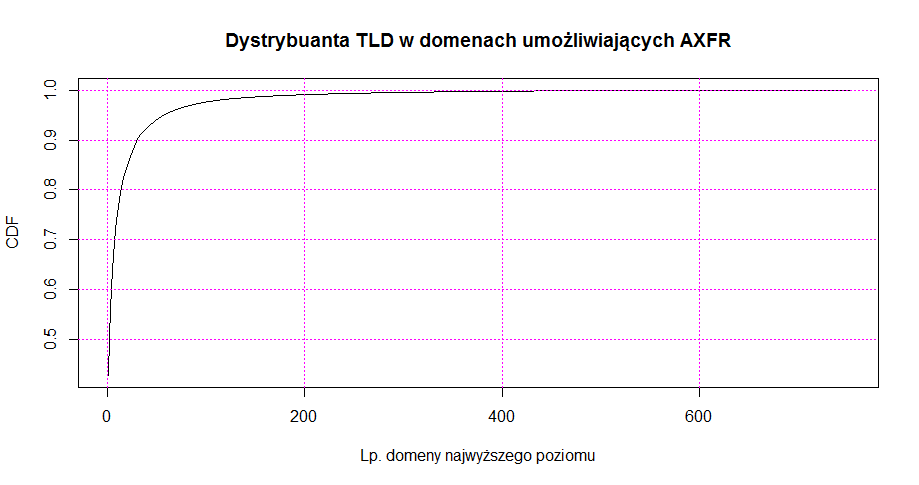
\includegraphics[width=1.0\textwidth]{image/cdf_tld_resp}
	\caption{}
	\label{cdf_tld_resp}
\end{figure}

\begin{table}[]
	\centering
	\caption{Opis zbiorów zapytań/odpowiedzi}
	\label{cdf_table}
	\begin{tabular}{|p{0.2\textwidth}|p{0.3\textwidth}|p{0.4\textwidth}|}
		\hline
		\textbf{Zbiór} & 
		\textbf{Liczba różnych TLD w zbiorze} & 
		\textbf{Liczba różnych TLD zawierająca 99\% elementów zbioru} \\
		\hline\hline
		Zapytania & 
		1521 & 
		147\\
		\hline
		Odpowiedzi & 
		751 & 
		187\\
		\hline\hline		
	\end{tabular}
\end{table}

Oprócz wykreślonych charakterystyk policzono również ile domen najwyższego poziomu gromadzi w sobie 99\% zapytań bądź odpowiedzi (w zależności od badanego zbioru). Wyniki zaprezentowano w tablei \ref{cdf_table}. Warto zauważyć, że pomimo ponad dwukrotnie mniejszego zbioru różnych domen poziomu najwyższego, należy zgrupować dużo więcej TLD aby uzyskać zbiór 99\% wszystkich odpowiedzi. Można z tego wnioskować, że rozkład odpowiedzi jest bardziej jednostajny niż w przypadku danych wejściowych. Można także przypuszczać, że zbiór wejściowy zawierał pojedyncze domeny z różnych, rzadko spotykanych TLD. W momencie, kiedy jedna, czy jedynie kilka domen z takiego TLD są odpowiednio zabezpieczone przed nieuprawnionym transferem AXFR nie znajdziemy danego sufiksu w zbiorze odpowiedzi. Sytuacja taka może mieć miejsce, gdy wszystkie domeny z mało popularnego TLD znajdują się pod zarządem jednej osoby czy organizacji.


\section{Analiza AS}
Podstawową informacją, którą uzyskać można wykorzystując pobrane dane z transferów AXFR jest przynależność otrzymanych adresów IP do konkretnych grup autonomicznych. Grupy te określają przynależność do sieci, które zarządzane są przed tego samego operatora sieciowego, a wykorzystuje się je głównie w protokołach routingu. Informacje związane z systemami autonomicznymi można, w głównej mierze, zanleźć w RFC1930\cite{RFC1930}.

